\graphicspath{{images/}}
\section*{LGS und Matrizen}

\subsection*{Matrizen}

\begin{definition}{Matrix}
    Tabelle mit $m$ Zeilen und $n$ Spalten.
    \begin{itemize}
        \item $m \times n$-Matrix
        \item $a_{ij}$: Element in der $i$-ten Zeile und $j$-ten Spalte
    \end{itemize}
\end{definition}

\begin{definition}{Transponierte Matrix}
    \begin{itemize}
        \item $A^T$: Spalten und Zeilen vertauscht
        \item $(A^T)_{ij} = A_{ji}$
    \end{itemize}
\end{definition}

\begin{minipage}{0.5\linewidth}
\begin{formula}{Addition und Subtraktion}
    \begin{itemize}
        \item $A + B = C$
        \item $c_{ij} = a_{ij} + b_{ij}$
    \end{itemize}
\end{formula}
\end{minipage}
\begin{minipage}{0.48\linewidth}
\begin{formula}{Skalarmultiplikation}
    \begin{itemize}
        \item $k \cdot A = B$
        \item $b_{ij} = k \cdot a_{ij}$
    \end{itemize}
\end{formula}
\end{minipage}

\begin{formula}{Matrixmultiplikation} $A^{m \times n}$, $B^{k \times n}$\\
    \begin{minipage}{0.6\linewidth}
    Bedingung: $A$ hat $n$ Spalten und $B$ hat $n$ Zeilen.\\
    Resultat: $C$ hat $m$ Zeilen und $k$ Spalten.
    \begin{itemize}
        \item $A \cdot B = C$
        \item $c_{ij} = a_{i1} \cdot b_{1j} + a_{i2} \cdot b_{2j} + \ldots + a_{in} \cdot b_{nj}$
        \item $A \cdot B \neq B \cdot A$
    \end{itemize}  
    \end{minipage}
    \begin{minipage}{0.35\linewidth} 
    \begin{center}
    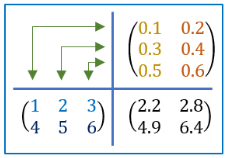
\includegraphics[width=0.8\linewidth]{matrixmultiplikation.png}
    \end{center}
    \end{minipage}
\end{formula}

\subsection*{Lineare Gleichungssysteme (LGS)}

\begin{concept}{Zeilenstufenform (Gauss)}
    \begin{itemize}
        \item Alle Nullen stehen unterhalb der Diagonalen, Nullzeilen zuunterst
        \item Die erste Zahl $\neq 0$ in jeder Zeile ist eine führende Eins
        \item Führende Einsen, die weiter unten stehen $\rightarrow$ stehen weiter rechts
    \end{itemize}
    \textbf{Reduzierte Zeilenstufenform: (Gauss-Jordan)}\\
    Alle Zahlen links und rechts der führenden Einsen sind Nullen.
\end{concept}

\begin{theorem}{Rang einer Matrix}\\
    Anzahl linear unabhängiger Zeilen- oder Spaltenvektoren.\\
    Rang $rg(A)$ einer Matrix $A^{m \times n}$:
    $$rg(A) = \text{Anzahl Zeilen - Anzahl Nullzeilen}$$
    \begin{itemize}
        \item Lösbar: $rg(A) = rg(A|b)$
        \item Nicht lösbar: $rg(A) \neq rg(A|b)$
        \item genau eine Lösung: $rg(A) = n$
        \item unendlich viele Lösungen: $rg(A) < n$
    \end{itemize}
\end{theorem}

\begin{KR}{Parameterdarstellung} bei unendlich vielen Lösungen
    \begin{itemize}
        \item Führende Unbekannte: Spalte mit führender Eins
        \item Freie Unbekannte: Spalten ohne führende Eins
    \end{itemize}
    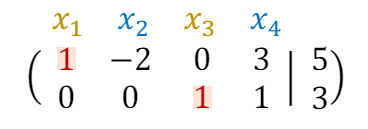
\includegraphics[width=0.3\linewidth]{parameterdarstellung_lgs.png}\\
    Auflösung nach der führenden Unbekannten:
    \begin{itemize}
        \item $1 x_1 - 2 x_2 + 0 x_3 + 3 x_4 = 5 \quad x_2 = \lambda \rightarrow x_1 = 5 + 2 \cdot \lambda - 3 \cdot \mu$
        \item $0 x_1 + 0 x_2 + 1 x_3 + 1 x_4 = 3 \quad x_4 = \mu \rightarrow x_3 = 3 - \mu$    
    \end{itemize}
    \vspace*{2mm}
    $$ \vec{x} = \begin{pmatrix} x_1 \\ x_2 \\ x_3 \\ x_4 \end{pmatrix} 
    = \begin{pmatrix} 5 + 2 \lambda - 3 \mu \\ \lambda \\ 3 - \mu \\ \mu \end{pmatrix} 
    = \begin{pmatrix} 5 \\ 0 \\ 3 \\ 0 \end{pmatrix} + \lambda \begin{pmatrix} 2 \\ 1 \\ 0 \\ 0 \end{pmatrix} + \mu \begin{pmatrix} -3 \\ 0 \\ -1 \\ 1 \end{pmatrix}$$
\end{KR}

\subsection*{Quadratische Matrizen}

\begin{formula}{Matrizen umformen}
    bestimme die Matrix $X$:
    $$A \cdot X + B = 2 \cdot X$$
    \begin{itemize}
        \item $A \cdot X=2 \cdot X-B$
        \item $A \cdot X-2 \cdot X=-B$
        \item $(A-2 E) \cdot X=-B$
        \item $(A-2 E) \cdot(A-2 E)^{-1} \cdot X=(A-2 E)^{-1} \cdot-B$
        \item $X=(A-2 E)^{-1} \cdot-B$
    \end{itemize}
\end{formula}

\subsubsection*{Inverse}

\begin{definition}{Inverse einer quadratischen Matrix $A$}
    \begin{itemize}
        \item $A \cdot A^{-1} = A^{-1} \cdot A = E$
        \item $A^{-1}$ existiert, wenn $rg(A) = n$
    \end{itemize}
\end{definition}

\begin{theorem}{Inverse einer $2 \times 2$-Matrix}\\
    \begin{minipage}{0.45\linewidth}
    $$A = \begin{pmatrix} a & b \\ c & d \end{pmatrix}$$
    mit $det(A) = ad - bc$
    \end{minipage}
    \begin{minipage}{0.5\linewidth}
        $$A^{-1} = \frac{1}{\det(A)} \cdot \begin{pmatrix} d & -b \\ -c & a \end{pmatrix}$$
        NUR Invertierbar falls $ad - bc \neq 0$
    \end{minipage}
    
\end{theorem}

\begin{KR}{Inverse berechnen} einer quadratischen Matrix $A^{n \times n}$
    $$A \cdot A^{-1} = E \rightarrow \left( A | E \right) \leadsto \text{Zeilenoperationen} \leadsto \left( E | A^{-1}\right)$$
\end{KR}

\begin{example}
    $$
\underbrace{\left(\begin{array}{ccc}
4 & -1 & 0 \\
0 & 2 & 1 \\
3 & -5 & -2
\end{array}\right)}_{A} \cdot \underbrace{\left(\begin{array}{lll}
x_{1} & y_{1} & z_{1} \\
x_{2} & y_{2} & z_{2} \\
x_{3} & y_{3} & z_{3}
\end{array}\right)}_{A^{-1}}=\underbrace{\left(\begin{array}{lll}
1 & 0 & 0 \\
0 & 1 & 0 \\
0 & 0 & 1
\end{array}\right)}_{E}$$
$$ \rightarrow\left(\begin{array}{ccc|ccc}
4 & -1 & 0 & 1 & 0 & 0 \\
0 & 2 & 1 & 0 & 1 & 0 \\
3 & -5 & -2 & 0 & 0 & 1
\end{array}\right)
$$

Zeilenstufenform (linke Seite)

$$ \leadsto 
\left(\begin{array}{ccc|ccc}
1 & -1 / 4 & 0 & 1 / 4 & 0 & 0 \\
0 & 1 & 1 / 2 & 0 & 1 / 2 & 0 \\
0 & 0 & 1 & -6 & 17 & 8
\end{array}\right)
$$

Reduzierte Zeilenstufenform (linke Seite)

$$ \leadsto 
\left(\begin{array}{ccc|ccc}
1 & 0 & 0 & 1 & -2 & -1 \\
0 & 1 & 0 & 3 & -8 & -4 \\
0 & 0 & 1 & -6 & 17 & 8
\end{array}\right) \Rightarrow A^{-1}=\left(\begin{array}{ccc}
1 & -2 & -1 \\
3 & -8 & -4 \\
-6 & 17 & 8
\end{array}\right)
$$
\end{example}



\begin{concept}{LGS mit Inverse lösen}
    $A \cdot \vec{x} = \vec{b}$
    $$A^{-1} \cdot A \cdot \vec{x} = A^{-1} \cdot \vec{b} \rightarrow \vec{x} = A^{-1} \cdot \vec{b}$$
    \textbf{Beispiel:}\\
    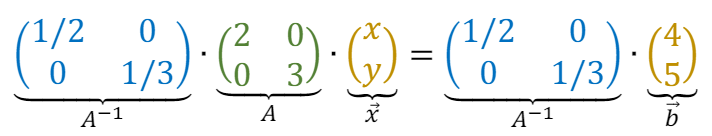
\includegraphics[width=0.5\linewidth]{lgs_inverse.png}
\end{concept}



